\chapter{Introduction}
\label{chap:Intro}
\vspace{-1em}
\epigraph{
  \textit{Machines were mice and men were lions, once upon a time. But now that it's the opposite, it's twice upon a time.}
}{Moondog \cite{Moondog}}
%


For most of the post-war era, the neutrino has been an unwanted guest in the house party of particle physics, the sort of person who is prone to spill unexpected experimental results on the carpet of theory not once, but time and again. However, one can hardly fault it; it was first invited to the party only reluctantly, in order to save one of the most cherished laws in physics --- that of momentum conservation. Beginning in the early 1900, experiments investigating the spectrum of $\beta$-decay (also referred to as a neutron decay) had a puzzling result; the two particles that were known, the proton and the electron, had a continuous, rather than discrete, kinetic energy spectrum. 

\section{Initial Discovery}
\subsubsection{Beta Decay and the Neutrino}
For ordinary one $\rightarrow$ two body decays, like what was being observed in the $\beta$-decay-  $n \rightarrow p + e^{-} $, momentum conservation requires that the momentum of the two daughter particles must cancel out, leaving only the initial momentum of the mother. Moreover, one of the daughter particles, the proton, is much more massive than its counterpart, meaning that the majority of the momentum from the interaction will be transferred to the proton. To be explicit-
\begin{eqnarray}
p_{net}= p_{proton} +p_{e^-} =0\\
E_{inital}= 0 \rightarrow \frac{p^2_{e^-}}{2m_{e^-}} +\frac{p^2_{proton}}{2m_{proton}} = E_{decay}\\
\frac{p^{2}_{e^-} \cdot (m_{e^-}+m_{proton})}{2m_{proton} \cdot m_{e^-}} = E_{decay} \\
p_{e^-} = \sqrt{\frac{E_{decay} \cdot 2m_{proton} \cdot m_{e^-}}{(m_{e^-}+m_{proton})}}
\end{eqnarray} 
meaning that the observed kinetic energy of the outgoing electron should show a discrete peak associated with the energy of the decay. However, what was observed was rather different; namely,  a continuous kinetic energy spectrum \cite{Beta_Spectrum} rather than the expected discrete peak. 

Many explanations to this troubling problem were offered, notably: a weakening of the law of conservation of energy, proposed by Bohr, which would require energy to only be conserved in aggregate, or a new, charge-less subatomic particle, proposed by Fermi in a 1930 letter \cite{Fermi}. Initially termed a neutron, (though its name was quickly changed to ``neutrino,'' little neutral one, after the discovery of the more massive neutron) this particle was postulated to be neutral in charge, $1/2 \hbar$ in spin, and in possession of only a very small mass. This would save the law of conservation of energy, but at a terrible price, as detecting this particle would be incredibly difficult; as Pauli joked, ``I have done a terrible thing, I have postulated a particle that cannot be detected.'' \cite{Pauli} A gloomy statement indeed, but not entirely inaccurate. It took until 1956 for the neutrino to be detected by the experiment of Cowan, Reines, \emph{et al} \cite{Cowan}. 

\section{First Detection}
  The experimental detection of the neutrino required an attack from many directions. First, and perhaps most importantly, a massive source of neutrinos was required to overcome the intrinsic low cross section of the weak neutrino interaction. Second, the experiment would require a signature that was unambiguous, to ensure that backgrounds from the reactor did not drown out the neutrino signal in a sea of noise. The solutions that were hit upon were used by many subsequent neutrino experiments. 
 
 To resolve the first issue, Cowan placed the neutrino detector close to a nuclear reactor, as the number of neutrinos generated from even a small nuclear reactor far outnumber those that could be generated from a strong radioactive source. The neutrinos (or, to be more precise, anti-neutrinos) that were generated from beta decay in the nuclear reactor would be detected in the inverse reaction of what initially prompted the postulation of the neutrino, the inverse beta decay $p + \bar{\nu} \rightarrow e^{+} + n$. The positron from this reaction would annihilate with electrons present in the target, generating a pair of $\gamma$s, which in turn would generate a large number of photons as a result of the scintillating material present in the target.  These photons would be detected with photomultiplier tubes: high sensitivity, fast read-out, low deadtime, photon detectors.
 
 Their initial signal was ambiguous, so their second innovation was to dope the target with a neutron-absorbing material, allowing for a double signal of prompt positron annihilation and delayed neutron capture. The material that they used to generate the neutron capture signal was Cadmium, which reacted via $ n+ ^{108}$Cd $\rightarrow ^{109m}$Cd $ \rightarrow ^{109}$Cd $+ \gamma$.  The two innovations --- the double signal and the large neutrino flux are still the basis for many modern neutrino experiments, such as Double Chooz, an experiment that will be discussed in more detail later. 


\section{The Solar Neutrino Problem}
The 1960's brought two major changes to the understanding of the neutrino: one long-expected and the other a rude shock. The former was the detection of the muon neutrino in 1962 by Lederman \emph{et al} \cite{Lederman}. First predicted as a result of observed muon decay $\mu \rightarrow \nu_{\mu} + \bar{\nu_{e}} + e^-$  which had a single easily observable product, but the spectrum of a 3-body decay. The delay in the muon neutrino's detection was caused by difficulty of producing heavy mesons. 

The development of the Alternating Gradient Synchrotron (AGS) allowed for the creation of large numbers of $\pi$ mesons, which decay into a muon and a muon neutrino via $\pi^{-} \rightarrow \mu^{-} + \bar{\nu_{\mu}}$. With a suitable shield  (in the case of AGS, a massive steel shield made from discarded battleship hulls) the muons were stopped before the target region --- a series of sequential neon-filled spark chambers --- while the neutrinos sailed through in their ghostly way. 

By sending a staggeringly large ($10^{14}$) number of neutrinos through the target, some small fraction interact with the neon to produce muons again, triggering the spark chamber and allowing for a photograph of the produced track. The experiment had a total live-time of 6 seconds, during which only 51 of the muon neutrinos were observed. Nevertheless, this Nobel-prize-winning experiment proved the existence of the muon neutrino and helped to cement the parallelism of the leptonic particles. 

At around the same time, much work was being done on the development of solar models. The standard solar model of Bahcall \cite {bahcall_intro_95} was developed to explain most of the observed physics of the sun. These models were, however, very sensitive to the exact nature of the reactions going on in the solar core, a region unobservable to standard astronomical techniques. Photons generated in the core of the sun are not observable, as they must pass through the solar surface --- an enormous amount of hot, dense gas opaque to photons.

Neutrinos offered a powerful tool to pull apart the problem, as they were directly produced by the reactions in the core, and were able to pass through the rest of the sun to reach earth-based detectors without being absorbed and re-emitted, as photons are. To observe these neutrinos the Homestake experiment was proposed and developed by Ray Davis and John Bahcall. Essentially a giant (100, 000 gallon or 380 cubic meters) tank of dry cleaning fluid (rich in chlorine), the experiment was located deep underground at the Homestake gold mine in the town of Lead, South Dakota. 

The experiment was designed to measure solar neutrinos via interactions with chlorine --- $\nu_e + ^{37}$Cl$ \rightarrow ^{37}$Ar$ + e^-$. The argon is then recovered from the detector and counted, giving the total number of neutrino interactions. Since the argon is recovered from the detector periodically, there's no good technique to filter out cosmic ray (or other) backgrounds, necessitating the extreme depth of the experiment. 

Despite the care taken in the experiment, the initial results were somewhat disappointing; approximately one-third of the predicted neutrino flux was observed in the detector \cite{Homestake}. At first, this was assumed to be a result of an undercount in the number of argon atoms in the detector, but, after bubbling argon through the detector and checking the argon generation rate through the deployment of calibration sources, the experiment was found to be making an accurate count of the number of argon atoms, and thus, the neutrino flux through the detector. 

The mystery of why the solar neutrino flux measured by Homestake (and, later, other experiments) was far in deficit of the expected result became known as the ``solar neutrino problem," and was the subject of intense speculation. Either the standard solar model was wrong, or there were some new physics in the neutrino sector. 

Naturally, initial investigations centered around changing the standard solar model. However, data gained from helioseismology suggested that the standard solar model was correct about the basic structure of the core of the sun \cite{Haxton}. Even stranger,  the neutrino flux results from Homestake seemed in direct opposition to the neutrino spectrum results of experiments like Kamiokande. 

Kamiokande, or more properly, Kamiokande II was a water Cherenkov detector. Initially designed to search for proton decay, it was re-designed to measure the solar neutrino flux through neutrino scattering on electrons. Though the cross-section for this reaction is small, the sheer volume of the Kamiokande-II detector meant that some of these reactions would occur. Moreover, Cherenkov radiation signals impose a clear directionality on neutrino interactinos, which allowed the detector to point back towards the source of the signal. Additionally, the detector was, unlike the radiochemical detector used by Homestake, capable of determining the energies of the neutrinos that it detected. 

By examining the solar neutrino spectrum, the experiment was able to get a rough measure of the physics going on inside of the sun. These results were incompatible with the reduced temperature changes proposed to the standard solar model as a result of the Homestake experiment. Moreover, the total neutrino flux measured by Kamiokande was half of that expected by the standard solar model, rather than the third of expected flux measured by the radio-chemical Homestake experiment. 

\section{Resolution of the Solar Neutrino Problem}

Something deep and mysterious was afoot in the neutrino sector. To untangle this mystery, however, further knots needed to be added in the form of an atmospheric neutrino deficit. In addition to looking at solar neutrinos, Kamiokande II was also engaged in measuring atmospheric neutrino ratios. Atmospheric neutrinos are generated by high energy cosmic rays in the upper atmosphere interacting with N and O nuclei,  producing kaons and pions. These particles  proceed to decay via:
\begin{eqnarray}
 \pi^{\pm} (K^{\pm}) \rightarrow \mu^{\pm} + \nu_{\mu}(\bar{\nu_{\mu}})\\
 \mu^{\pm} \rightarrow e^{\pm} + \nu_e(\bar{\nu_e}) + \bar{\nu_{\mu}}(\nu_{\mu})
 \end{eqnarray} 

Therefore, the ratio of $\nu_{e}$ to $\nu_{\mu}$ (including both neutrinos and antineutrinos) should approach 1:2. However, when the ratio was measured by Kamiokande II, it was found to be about 0.6 of the expected value \cite{SuperK}. Something had to be causing an overproduction of some neutrino species and an underproduction of others. One proposal for the solution of this issue was to borrow the concept of flavor mixing from the quark sector and use it for neutrinos, such that neutrinos produced in one flavor would oscillate into other flavors. 

Since the sun was assumed to produced almost exclusively electron-flavor neutrinos, solar neutrino experiments to date had been designed to detect electron neutrinos, rather than being sensitive to all the three different neutrino flavors. Therefore, a detector sensitive to all three neutrino flavors would be able to detect the true solar flux, and confirm the oscillation hypothesis. 

Initial hints of the confirmation of this hypothesis came from the upgraded Super Kamiokande Detector in 1998, when it found evidence of neutrino oscillations in atmospheric neutrinos. This result was rapidly followed by the confirmation of solar neutrino oscillations from the Sudbury Neutrino Observation (SNO), a heavy water neutrino detector in Canada. SNO, like the Kamiokande experiment, was based around use of Cherenkov light to detect neutrinos. However, because the heavy water used by SNO, it was able to view neutral current interactions of the form: $\nu_{x} + ^{2}$H $\rightarrow N + P + \nu_{x}$,  unlike the Kamiokande experiment, making it sensitive to neutrino interactions of all flavors. SNO's measurements of the total neutrino flux confirmed the standard solar model \cite{SNO}, while the proportionality of the three flavors confirmed neutrino oscillation as the explanation for the solar neutrino problem. A graph of this can be seen in Fig. \ref{Neutrino_Problem}.

\begin{figure}
\caption{Standard Model predictions of neutrino flux compared to experimentally observed rates, showing a deficit \cite{Bahcall}.}
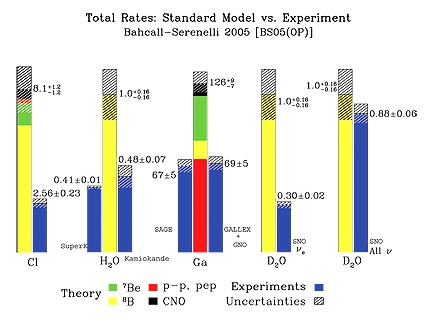
\includegraphics[width=\textwidth]{tex/colortheoryvsexp.jpg}
\label{Neutrino_Problem}
\end{figure}


\section{Neutrino Oscillation and the PMNS Matrix}
Neutrino oscillations were originally developed by Pontecorvo in the late 1950's as a way of characterizing the uncertain Majorana nature of the neutrino \cite{Ponte}. This idea was expanded by Maki, Nakagawa, and Sakata in the 1960's, creating a mathematical framework to handle neutrino flavor oscillations, CP phase violations, and the Majorana ``angle'' of the neutrino \cite {PMNS}. 

The PMNS (Pontecorvo, Maki, Nakagawa, Sakata) matrix is a unitary ``rotation" matrix which acts on a vector in the mass basis ($\nu_{1} \nu_{2} \nu_{3}$) to transform it into the flavor basis  ($\nu_{e} \nu_{\mu} \nu_{\tau}$) , i.e.

\begin{equation}
 \left(\begin{matrix}
  \ket{\nu_e} \\ \ket{\nu_{\mu}} \\ \ket{\nu_{\tau}}
 \end{matrix}\right) =  
\left(\begin{matrix}
  U_{e1}& U_{e2} &U_{e3}\\ 
U_{\mu1} &U_{\mu2} &U_{\mu3}\\ 
U_{\tau1}& U_{\tau2}& U_{\tau3}\\ 
 \end{matrix} \right)
\times\left(
 \begin{matrix}
  \ket{\nu_1} \\ \ket{\nu_2} \\ \ket{\nu_{3}}
 \end{matrix}\right)
\end{equation}

The unitary matrix (U above) is the PMNS matrix,  and can be decomposed into a trio of rotations matrices and a Majorana matrix \cite {PMNSBreakdown}. 

\begin{equation}
 U=\left(\begin{matrix}
    1&0&0\\
0&c_{23}&s_{23}\\
0&-s_{23}&c_{23}
   \end{matrix}\right)
\times
\left(\begin{matrix}
    c_{13}&0&s_{13}e^{-i\delta_{CP}}\\
  0&1&0\\
-s_{13}e^{i\delta_{CP}}&0&c_{13}
   \end{matrix}\right)
\times
\left(\begin{matrix}
    c_{12}&s_{12}&0\\
-s_{12}&c_{12}&0\\
0&0&1
   \end{matrix}\right)
\times
\left(\begin{matrix}
    e^{i\phi_1} & 0 & 0 \\
0 & e^{i\phi_2} & 0 \\
0 & 0 & 1
   \end{matrix}\right)
\end{equation}

In the equations above, the \emph{$c_{xy}$} and \emph{$s_{xy}$} terms are sines and cosines of the neutrino mixing angles $\theta_{xy}$, while the $\delta$ is the CP-violating phase and the $\phi$ is an adjustable parameter to account for the Majorana-ness of the neutrino. Specifically, the neutrino is not prohibited by experiments from acting as its own anti-particle. If a neutrino is a Majorana particle (able to act as its own anti-particle) it will have a Majorana phase and the term $\phi$ will be non-zero.  Similarly, if there was no neutrino flavor mixing, the $\theta_{xy}$ terms would be zero. However, the neutrino flavor mixing angles are known to be non-zero, and can be experimentally determined by measuring the appearance and disappearance of neutrino flavors.

To be more precise, neutrinos are produced as a result of weak interactions, forcing the neutrino into a known flavor eigenstate. Since the neutrino is in a flavor eigenstate, the mass eigenstate is a linear combination of all three values. As the neutrino propagates, it can be treated as a plane wave of the form

\begin{equation}
 \mid \Psi_i (t) \rangle  =  e^{ -i(E_{i}  \cdot t - \overrightarrow{p_{i}} \cdot \overrightarrow{x}) } \mid \Psi_i (0) \rangle
 \end{equation}

In the relativistic limit, this equation reduces to 

\begin{equation}
 \mid \Psi_i (L) \rangle  =  e^{\frac{-im_i L}{2E}} \mid  \Psi_i (0) \rangle
 \end{equation}

Therefore, the probability of a neutrino changing flavor between creation and detection can be expressed as 
\begin{equation}
P_{a \rightarrow b} = \mid \langle \Psi_b \mid \Psi_a (t) \rangle \mid^2 \\
= \mid \sum_{i} U^{*}_{ai} U_{bi}e^{\frac{-im_i L}{2E}} \mid ^2
\end{equation}
where U is the unitary mixing matrix discussed previously.  

It is at this point that we leave the realm of historical overview, and enter into the world of modern neutrino experiments, designed to measure the various parameters of the neutrino mixing matrix \emph{U}. One particular experiment, Double Chooz will form the core of thesis. 

\section{Chapter Overview}
This thesis is broken into three primary chapters, in addition to this introduction. The contents of each chapter are addressed in turn, beginning with the chapter discussing the Double Chooz neutrino mixing experiment. This is followed by a chapter focusing on our unique contribution to the Double Chooz experiment, a the articulated arm calibration device. Finally, the thesis turns to a search for paraphotons, a light, neutral, axion-like particle in the Double Chooz 3rd publication data set. 

\subsubsection{The Double Chooz Experiment and the Search for $\theta_{13}$}
In Chapter \ref{chap:Double Chooz}, the thesis discusses of Double Chooz experiment, and the results of its search for the mixing angle $\theta_{13}$. However, the groundwork must first be laid; the chapter begins with a discussion of the physical experiment, as well as the software tools that have been developed to assist in the analysis of Double Chooz data. The experimental performance of the detector is then discussed, as well as a brief mention of the results of other modern $\theta_{13}$ searches. 


\subsubsection{The Articulated Arm and Full-Volume Calibration of the Double Chooz Experiment}
In Chapter \ref{chap:AA} we will discuss the articulated arm, a full volume calibration system developed for the Double Chooz experiment. Despite the success of Double Chooz, there are improvements that can be made to the accuracy of the detector. One of the most striking areas that can be improved is the ability of the experiment to accurately reconstruct neutrino position inside the detector and improve sensitivity of the $\theta_{13}$ final measurement in Double Chooz. To this end, a full-volume calibration device was constructed, tested, and deployed in the far detector of Double Chooz. The development, simulation, and results of the device are detailed in this chapter. 


\subsubsection{Paraphotons}
In Chapter \ref{chap:Paraphotons} we will discuss use of the Double Chooz detector to observe paraphotons. Paraphotons are heavy bosons generated by a U(1) extension of the standard model, an extension motivated by some anomalous results from astronomical observations. The paraphoton also helps to explain the light mass of the observed neutrino flavors. This chapter will briefly cover the theory of the paraphoton, as well as the use of Double Chooz to detect them, and the results of a search for them in the Double Chooz 3rd publication dataset. 